\documentclass[12pt]{article}
\usepackage{graphicx}
\graphicspath{ {images/} }  
\usepackage{fixltx2e}
\usepackage{booktabs}	  
\usepackage{float}         		

\title{An efficient query platform for streaming and dynamic natural graphs}
\author{Milindu Sanoj Kumarage}							

\begin{document}

\begin{titlepage}

\newcommand{\HRule}{\rule{\linewidth}{0.5mm}} % Defines a new command for the horizontal lines, change thickness here

\center % Center everything on the page
 
%----------------------------------------------------------------------------------------
%	HEADING SECTIONS
%----------------------------------------------------------------------------------------

\textsc{\Large SCS4124}\\[0.5cm] 
\textsc{\large Final Year Research in Computer Science}\\[1.5cm]
\textsc{\LARGE Proposal}\\[0.5cm] 
%----------------------------------------------------------------------------------------
%	TITLE SECTION
%----------------------------------------------------------------------------------------

\HRule \\[0.4cm]
{ \LARGE \bfseries An efficient query platform for streaming and dynamic natural graphs }\\[0.4cm]
\HRule \\[1.5cm]
 
%----------------------------------------------------------------------------------------
%	AUTHOR SECTION
%----------------------------------------------------------------------------------------

\begin{minipage}{0.4\textwidth}
\begin{flushleft} \large
\emph{Author:}\\
Milindu Sanoj Kumarage\\
12000752\\
\end{flushleft}
\end{minipage}
~
\begin{minipage}{0.4\textwidth}
\begin{flushright} \large
\emph{Supervisor:} \\
Dr.D.N. Ranasinghe
\end{flushright}
\end{minipage}\\[4cm]

% If you don't want a supervisor, uncomment the two lines below and remove the section above
%\Large \emph{Author:}\\
%John \textsc{Smith}\\[3cm] % Your name

%----------------------------------------------------------------------------------------
%	DATE SECTION
%----------------------------------------------------------------------------------------

{\large \today}\\[3cm] % Date, change the \today to a set date if you want to be precise

%----------------------------------------------------------------------------------------
%	LOGO SECTION
%----------------------------------------------------------------------------------------

%\includegraphics{Logo}\\[1cm] % Include a department/university logo - this will require the graphicx package
 
%----------------------------------------------------------------------------------------

\vfill % Fill the rest of the page with whitespace

\end{titlepage}
 

\tableofcontents

\clearpage 
\section{Preface}

This document is the proposal for the 4th Year Individual Project for partial fulfilment of
the requirements of the Degree of Bachelor of Science in Computer Science, at University of
Colombo School of Computing, University of Colombo, Sri Lanka.
This proposal provides the scope and context of the project to be undertaken It details
the objectives of the research, research questions, background and research methodology.This
document also provides the project schedule, a description of anticipated results and the final
products.
The intended audience of this document is the academic staff of the University Of Colombo
School Of Computing and it is intended to enable them to determine whether the project should
be approved as proposed, approved with modifications, or not approved.
\\
[7em]
Milindu Sanoj Kumarage\\
[7em]
Dr.D.N. Ranasinghe\\

\clearpage 
\section{Motivation}

Massive scale datasets are getting common in day-to-day business with the expansion of the internet. More and more devices getting connected, more and more services coming online, more and more data generated and at the same time, the need to work on these data is getting more and more prominent.

However, modern day datasets no longer fit into one computing node as the amount of collected data are enormously huge.  We need some kind of a grid with thousands of computing nodes which can work on the dataset parallely, which might be distributed even across many geographical areas but connected through a network, communicating and coordinate their actions.

In the other hand, mapping these data into graphs and using graph algorithms to query useful information out of these graphs is also a growing need. Business intelligence systems, anomaly detections systems and many more real world use cases with huge financial values exists which needs insights that could be extracted from the relationships in the graphs, which is not easy to extract from traditional databases. We know the story of Google, how it became the search giant with their PageRank\cite{PageRank} algorithm which makes use of graph relations to rank the web pages of the World Wide Web and to produce the users the most related web pages to their queries. In the same way, Facebook uses their social graph with trillion edges\cite{Facebook} to uncover new insights about their users, products, and interactions.


With the popularity of the use cases like above, the need of betters platforms which can perform graph computations efficiently in parallel on largely distributed clusters aroused. Query platforms makes it easier to query for data and we have seen several query platforms popping up like HiveQL which runs on Hadoop, Spark SQL which runs on Apache Spark and Gremlin which is used by several graph databases like Neo4J and Titan. Query platforms are useful when the information needed to be retrieved is dynamic, for instance, a Business Intelligence tool needs different types of information represented in different ways.

Another example would social networks like Facebook, Twitter, etc where we get a Feed which shows selected set of posts to a particular user that is best matching for the user’s interests at a given moment, however, with the user’s interactions with these posts shown, user’s Feed start showing different set of posts which are more related to the posts the user is much interest in. This is a Pub/Sub system, where we get different subscribers with different needs over the publications stream and the subscription space dynamically changes over the time. We see even Facebook uses\cite{Facebook} Apache Giraph which is an open-source implementation of Pregel\cite{Pregel}, which does not take the characteristics of natural graphs into account, and which is not capable of working with streaming graphs. Therefore, motivation of this research is to improve performance in the case of streaming and natural graphs by exploiting their intrinsic characteristics.

\section{Research Aim and Research question}

\subsection{Aim and objectives}

Aim of this research is to introduce a model for a graph query platform which enables querying massive scale, streaming and dynamically changing natural and synthetic graphs. This model should be able to work on top of existing distributed storages and make use of existing distributed computation approaches.

We also try to apply our proposed model to solve top-k content based stream matching where pub/sub interactions interpreted as a streaming graph.
 
\subsection{Research Question}
The problem is to find a optimal model for a query platform, a graph framework which enables interacting with the graph, for a graph G, where the graph G is streaming, which implies that the graph is continuously growing by receiving the vertices and edges as a stream of data, and the graph G be natural, typically having power-law degree distributions which implies that a small subset of the vertices connects to a large fraction of the graph.

\clearpage 
\section{Introduction}

This section presents an overview of the research problem "Query platform for streaming and dynamic natural graphs" in concise, which includes an overview of natural graphs, examples of natural graphs from day-to-day life and practical applications, comparison of data-parallel and graph-parallel systems, graph partitioning, edge-cut method against vertex-cut method, graph sketching, graph modelling, etc.

\subsection{Natural graphs and Real-world examples}

Massive-scale graph-structured computation happens in many systems ranging from targeted advertising to natural language processing and has led to the development of several graph-parallel abstractions. 

One example of such system is social networks, like Facebook, Twitter where different types of interactions of users happens every second. According to the statistics, the number of active users on the Twitter social and micro blogging network is roughly 305 million by the fourth quarter of  year 2015\cite{TwitterStats}. We can map interactions of users into an unbounded graph, where the graph keeps building as long as users keeps using the social network.

Another example is web crawlers, where the crawler through the web pages following links in the given web page. We can map web pages to vertices and properties of a particular web page as attributes of a vertex. And then we can map hyper links from one web page to another as a edge between the relevant vertices.  

One another example would be Anomaly  Detection Systems, where the system monitor different types of data like HTTP traffic, System logs, etc and trying to analyse and find the anomalies using the relationship of the data by building a graph.

\begin{figure}
\centering
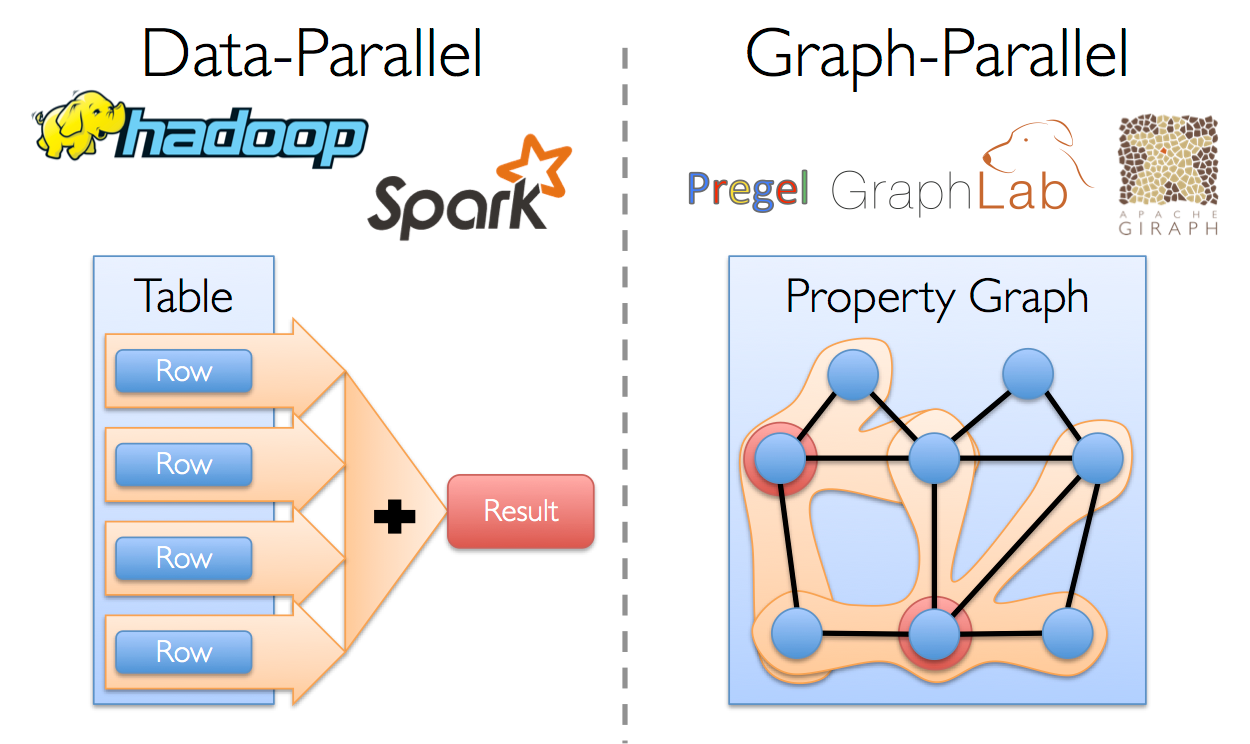
\includegraphics[width=\textwidth]{image00.png}
\caption{Difference between data-parallel and graph-parallel}
\label{fig:parallel}
\end{figure}

\subsection{Data-Parallel and graph-Parallel systems}

Data-parallel systems like Hadoop, Spark, Beam, etc threats the data as sets of records and do the parallel processing. Graph-parallel systems threats the data as a graph, where data get mapped to nodes and edges to represent the relationships between data. See Figure \ref{fig:parallel}. Some examples for graph-parallel systems are Pregel, GraphLab.

\subsection{Query Platforms}
Query platforms enables developers easily query data from the graph. We often see people use tools to run queries to fetch data on the fly. We see different type of query languages introduced for different needs. Hive SQL and Spark SQL are both for data-parallel systems while Gremlin is a query language in Apache TinkerPop stack which can be used for both graph databases (OLTP, Online transaction processing) and graph analytic systems (OLAP, online analytical processing). And we see systems like Apache Drill which is a schema-free SQL query engine for Hadoop, NoSQL and Cloud Storages. Building such a query platform needs different aspects taken into consideration. Partitioning, indexing , storage model, locking and edge compression are few of them. 

\subsection{Graph partitioning}

We have to accommodate graph partitioning methods to partition these generated massive-scale unbounded graphs to be assigned to  different computation nodes in order to do the analysis. Best partitions would be having less connections in between partitions, thus, will reduces the communication between partitions, which could be costly otherwise.

\subsection{Edge-cut and Vertex-cut methods}

Existing graph partitioning methods can be divided into two main categories, as edge-cut and vertex-cut methods. Edge-cut tries to evenly assign the vertices to machines by cutting the edges and vertex-cut tries to evenly assign the edges to machines by cutting the vertices. 

\subsection{Graph partitioning for Natural graphs}

However, the natural graphs commonly found in the real-world have highly skewed power-law degree distributions, which challenge the assumptions made by abstractions like  Pregel and GraphLab, limiting performance and scalability. As natural graphs are highly skewed, there exists subset of vertices which have large number of edges. 

For example, a common World Wide Web crawler would find most of the web pages have average number of hyper links pointing to them while some web pages have massive number of hyper links pointing to them. 

When we use edge-cut approach evenly distributing vertices could result some partitions with too many edges but when we use vertex-cut approach we get edges evenly distributed across the partitions, therefore no one partition would get too much load. Therefore, vertex-cut methods can achieve better performance than edge-cut methods\cite{PowerGraph} specially for graphs that follows power-law degree distribution.

\subsection{Indexing}
Indexing makes data readily accessible and querying faster. We see systems use in memory indexing for fast accessing. Vertex-centric indices are what Titan and OrientDB uses in their implementation, which is interested in edge properties, because they argue vertex centric indexes are an important tool for scaling graph databases.

\section{Methodology}

We will be researching with different types of graphs( synthetic and natural ) from different sources. Once such source would be interactions of users in a social network, like Twitter, where new vertices and edges keeps inserted as the user interactions keeps happening over the time. We can map Photos, Tweets, Lists, Users, Hashtags, etc as vertices on a graph and Upload, Tweet, Join, Belong, Follows, etc as edges connecting these vertices.

Another source would be a web crawler where we keep getting new vertices and edges while the web crawler is crawling through the web. We can map web pages, images, etc to vertices, their properties as attributes of vertices and links between them as edges. We can use a simple web crawler which traverse in the World Wide Web, starting from a given web page, then moving to other linked pages by following the hyper links. Properties of the web pages will be mapped as attributes of the vertices. While the crawler traverse the web pages, pages it can write to a stream of data, where we can map these data on a stream of vertices and edges. This is an unbounded graph since we do not know how large the graph would be and the graph keeps building while the crawler keeps traversing.

As the first step, we will be designing the architecture of the platform, having the top most layers as the interface for users to run their graph algorithms and the bottom most layers as the interface for persistence layer. Intermediate layers would be graph modelling, sketching, partitioning, etc. 
 
For this, we will be studying the current graph frameworks ( eg: GraphX, Gelly ), graph databases ( eg: Neo4J, Titan ), graph analysis systems( eg: Apache Giraph, Pregel), data streaming systems ( eg: Apache Spark, Apache Flink ), graph sketching techniques \cite{GraphSketches}, graph partitioning techniques \cite{PowerGraph} \cite{S-PowerGraph}, etc. We will be trying out the currently available solutions ( eg: graph databases, graph partitioning techniques, graph sketching techniques, etc ) and observe the performances and effectiveness. Statistics from these experiments would help us with our benchmarking against our own model. 

 Then we would try out to build our query platform with different approaches of partitioning, sketching, streaming, modelling, etc the graph to find out the most optimal and efficient ways. 
 
 Traditional graph query platforms works in "Think like a vertex" manner, however Giraph++ \cite{GiraphPlusPlus} suggests "Think like a graph" is better. We will be investigating if we can follow this method with graph sketches and how partitioning should be done.

We will be researching how we can introduce the new model to exploit the limitations of current systems and intrinsic characteristics of streaming natural graphs.

\begin{figure}[H]
\centering
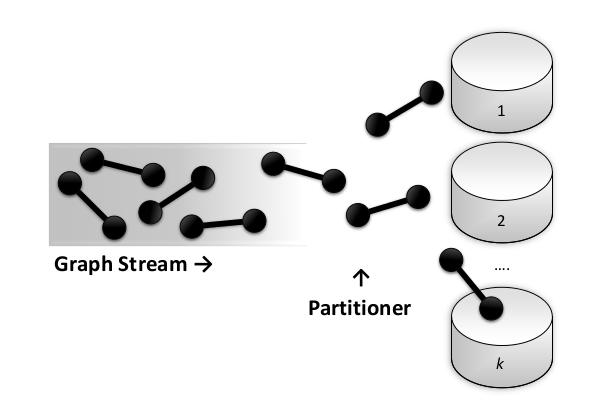
\includegraphics[width=\textwidth]{image01.png}
\caption{Partitioning the streaming vertices and edges into partitions }
\label{fig:partitioning}
\end{figure}

\clearpage 
\section{Anticipated Results / Final Products }
Final outcome of this research would be a better model for a query platform for streaming graph natural graphs. And statistical analysis with the performance of the proposed model against the existing graph frameworks. And a research thesis on the approaches the research followed and the obtained results with the approaches. 
 
\section{Delimitations and Scope}
Scope of the project limited to a model for a query platform which uses the existing distributed storages. We may or may not use any excising graph abstractions and graph algorithms.

\section{Literature Review}

We see several systems developed to cater the need of graphs related problems.

Apache Spark and its graph abstraction package GraphX\cite{GraphX} has gained lot of attention in the developer community for their graph based computational needs recently. GraphX also uses Pregel, but its own optimized variant of Pregel, in its underneath implementation.

And these systems uses different graph partitioning techniques. These techniques are base on various assumptions and have some limitations in some situations. There have been several researches done very recently and several papers published on the research problem on how to achieve better performance and how to avoid these limitations. 

\subsection{Static graphs}

\subsubsection{Pregel}

Pregel\cite{Pregel} graph framework was introduced for graph-parallel computations, where the computation is expressed as a sequence of steps, called 'supersteps'. In each step, a vertex receives a message from the previous step, changes its state and pass the message to the other vertices. Since Pregel is a synchronous system, it updates all parameters of vertices in parallel using values from the previous step as input. Partitioning of the graph is done by simply using a hash function on vertex ID. 

\subsubsection{GraphLab}

Then GraphLab\cite{Graphlab} \cite{DistributedGraphLab} was introduced for dynamic and asynchronous graph-parallel computation. GraphLab consists of a Data Graph which holds the program state, an Update Function, which is a stateless procedure, that updates the Data Graph in small chunks called Scopes and a Sync Function which concurrently maintains global aggregates. Different hash functions can be used to partition the graph. 

\subsubsection{DistributedGraphLab}

The Distributed GraphLab \cite{DistributedGraphLab} was to extend the GraphLab to fit to distributed environment.  

\subsubsection{Giraph}
Apache Giraph is one such graph processing system that is used at Facebook to analyse the social graph formed by users and their connections. It is an open-source implementation of Google’s Pregel\cite{Pregel} graph processing architecture. 

\subsubsection{Giraph++}
Giraph++\cite{GiraphPlusPlus} is an improved version of Apache Giraph, which is graph centric rather vertex centric. Main difference between Giraph and Giraph++ is, in Giraph++, the programmer can access the whole sub-graph in a partition, rather one vertex at a time. In Giraph++ each partition contains a set of vertices and all their outgoing edges. Each vertex is uniquely identified by an ID, and a partitioner decides which partition a vertex belongs to based on its ID. The partitioner is also used to route messages for a vertex correctly to its partition. The default partitioner is a hash function on the vertex ID.

\subsection{Streaming graphs}

\subsubsection{S-PowerGraph}

S-PowerGraph\cite{S-PowerGraph} discuss several methods as 'Degree', a greedy procedure which makes use of the in-degree distribution and 'DegreeIO' which tries to meet the challenge that both indegree and outdegree of natural graphs are skewed.

S-PowerGraph firstly suggests the Grid-based Constrained Random Vertex-cut algorithm of GraphBuilder\cite{Graphbuilder}  could be altered for streaming graph partitioning. In this method, a vertex is mapped into a shard which accommodates a constrained set of partitions. Then, the partition a vertex to be assigned will be chosen from the constrained set randomly. The edge e is assigned to P\textsubscript{idx} where idx is decided by idx = GridHash(e), the hash function implemented in GraphBuilder.

Then the S-PowerGraph discuss about an enhanced version of the greedy algorithm proposed in PowerGraph\cite{PowerGraph}. As the greedy algorithm in PowerGraph could lead to some unbalanced partitions in some cases, they introduce Balance(PowerGraph) where Balance() is a constraint to avoid the imbalance. 

\subsubsection{Apache Flink Gelly}
Apache Flink is a data stream processing framework and Flink's graph framework is Gelly. However, Gelly is only for static graphs. However, this \cite{Kalavri} is a research on how to extend to Gelly to support streaming. They have used Flink's shared states to continue the graph across iterations of the stream. 

\subsection{Graph partitioning}
\subsubsection{Fennel}

Fennel \cite{Fennel} is a one pass streaming graph partitioning technique which outperforms the de-facto standard offline software METIS on numerous real-world graphs, like Twitter graph with more than 1.4 billion of edges, which outputs balanced partitions.

\subsubsection{Linear Embedding}

"Distributed Balanced Partitioning via Linear Embedding"\cite{Linear Embedding} discusses a method researchers at Google have tried and tested with Google services. "Linear Embedding" is a balanced partitioning problem where the goal is to partition the vertices of a given graph into k parts so as to minimize the total cut size. Linear Embedding method first embeds nodes of the graph onto a line, then attempt to improve the ordering mainly by swapping vertices in a semi local manner and finally accommodate a post-processing method to improve the cut-size.

They discuss several different methods for each different step and compare the outcome performances for each combination. For embedding nodes onto a line,  they accommodate random mapping, Hilbert curve mapping when geographic/geometric information is available, and Affinity-based mapping which takes into account the affinity of vertices by grouping vertices that are closely connected, hence building a tree of these connections.

Once the linear embedding is done, the next step is to  improve ordering using semi local moves. One method is using Minimum Linear Arrangement (MinLA)\cite{MinLA} and the other is Rank Swap which depends on the pre chosen cut boundaries, the number of final partitions k. Finally they accommodate a post-processing method like dynamic programming to adjust the cut sizes.

\subsection{Graph sketching}
\subsubsection{TCM}
Sketching is process where we summarize a huge graph into a smaller graph, but we loose some data. Therefore we have to use different sketches for different types of queries. However, TCM is a research carried out for sketching which we can use for every types of queries. It uses hash buckets for sketching, and it not only sketch the edges, but also paths.

\subsection{Graph databases}

\subsubsection{Titan}
Titan is a distributed graph database engine build on top of Cassandra as the underlying data storage, but which now supports other data storage systems like HBase and BerkeleyDB. Titan natively supports the Gremlin Server component of the TinkerPop stack. Titan’s storage model is an adjacency list in a column family where row key is vertex id. Titan maintains indexes in a separate column family and one nice feature of Titan is we can accommodate third party tools like Elasticsearch, Lucene, etc for indexing.

\clearpage 
\section{Research design with high-level diagrams}

\subsection{Graph stream interface}
The users should be able to plug a stream of data to the systems, though a mapper which maps data into  edges and vertices and input to the graph model as a graph stream. 

\subsection{Graph model}
We can implement a graph in several ways, using linked list or a squire matrix are the popular options. We have to identify which method suits our needs and limitations. Some other options worth trying are non-square matrices which makes use of power low degree distribution of natural graphs. 

\subsection{Graph sketching}
Building a sketch of the graph makes us summarise the huge graph into a small model. There are many sketching techniques, some techniques limits the model for specific types of queries. We have to investigate good sketching techniques which does not limits us, and which suits well with the graph model ( linked list, squire matrix or non-square matrices ) we use and graph partitioning techniques we use. Figure \ref{fig:graph-sketching} shows how we can apply TCM \cite{TCM} model to sketch  graph. 

\begin{figure}[H]
\centering
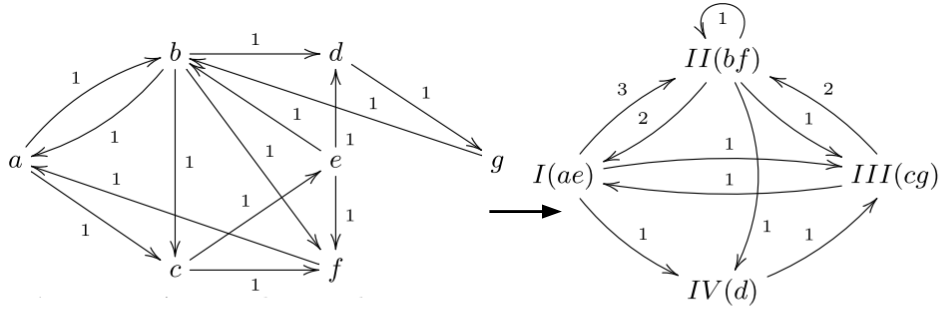
\includegraphics[scale=0.3]{graph-sketching.png}
\caption{Converting a graph into a TCM sketch}
\label{fig:graph-sketching}
\end{figure}

\subsection{Graph partitioning}
Partitioning depends on the above two factors, how we model the graph and how we sketch the graph. We have to find the best ways to minimize inter partition communication in order to obtain higher performance.

\subsection{Persistence interface}
We have to persist the data onto a storage and this should  be some persistence method which is familiar to the users. We could write to a Hadoop HDFS or to a database like Apache Cassandra.

\begin{figure}
\centering
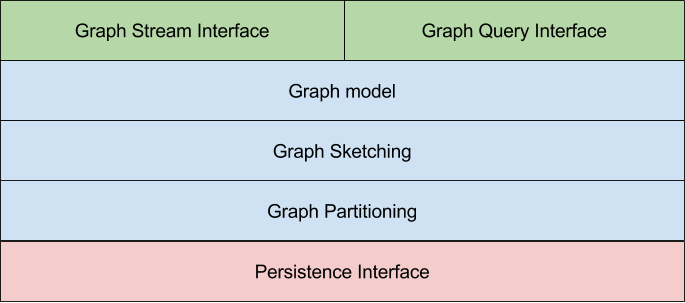
\includegraphics[scale=0.5]{intended-architecture.png}
\caption{Intended architecture of the platform}
\label{fig:web-graph}
\end{figure}

\clearpage 
\section{Preliminary results and discussion}

We first started implementing a streaming graph using a web crawler, which builds a web graph while crawling the web. We used  GraphStream, which is a Java library for the modeling and analysis of dynamic graphs, to visualize the generated web graph and analyse the degree distributions, etc. 

As you can see on the Figure \ref{fig:web-graph}, which is a snapshot of the generated web graph by the crawler, there are nodes with higher number of edges and, there are nodes with less number of edges.

\begin{figure}
\centering
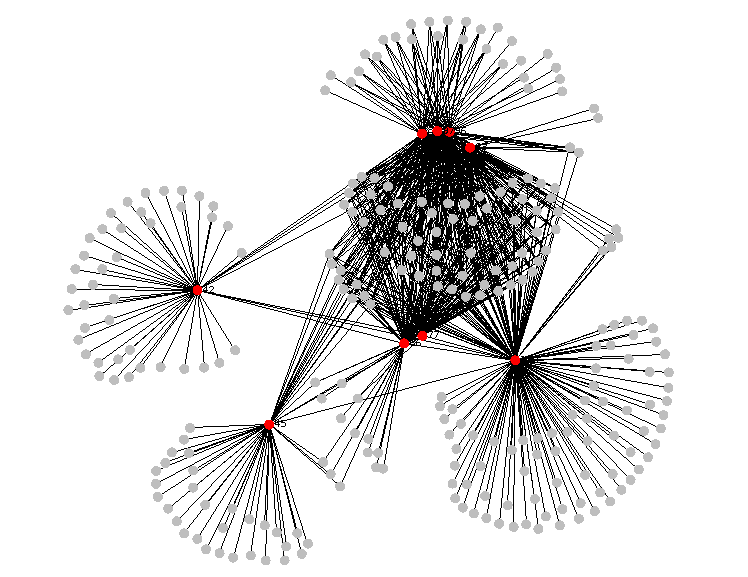
\includegraphics[scale=0.5]{web-graph.png}
\caption{Snapshot of the generated Web Graph}
\label{fig:web-graph}
\end{figure}

We then tried to build the Web graph using above web graph stream and Apache Spark's GraphX framework, however, we realized GraphX has no capability of working with streaming graphs. 

Then we moved on to Apache Flink, which is a relatively new streaming framework like Apache Spark, but not like Spark which is not truly real-time, but micro-batching based; Apache Flink as gained a lot of attention recently in the developer and research communities. Like Apache Spark, Flink is a streaming framework where we can plug different data streams and run different types of data analysis jobs on it. They too have a graph framework called Gelly, which run on top of Flink, like Apache Spark has GraphX.

However, same as GraphX, Gelly too is for static graphs. Fortunately, on of the researchers who as the same interest on graph streaming like us, has implemented a Gelly extension which can work with streaming graphs.

We then implemented a graph stream for Flink, using Twitter to build a social graph. Then we using the above extended Gelly framework, implemented the streaming graph. We then analysed the degree distributions of the graph time to time, as it grows. We realized there is a limitation in this scenario too. We can't dynamically submit any analysis on the building graph, but we have to pre define the analysis we need to do at the same time the graph start building. We communicated with the researcher who implemented the extension to Gelly about this and she confirmed it. 

Now, our next move is to take it further, try extend the Gelly to take analysis jobs on the run, while the graph keeps building. Furthermore, we are trying introduce graph sketching techniques and better partitioning techniques, then  analyse the performance gain.


\clearpage 
\section{Student’s personal statement} 
As a Final year Computer Science undergraduate my desire is to apply my knowledge in to solving this arising problem of efficient platform to interact with massive scale, natural graphs in streaming settings using a query language. This will benefit lot of software systems which works with massive scale graphs, like business intelligent systems which looks upon sales and production data for helping making better business decisions, internet of things systems which receives lot of inputs from millions of devices and send out commands to perform based upon the collected data from all the devices, and anomaly detection systems which monitors networks, trading systems, etc and try to detect the anomalies based upon the relationships between the data and the list continue on.  

\clearpage
\begin{table}[]
\centering
\caption{Project timeline}
\label{project-timeline}
\begin{tabular}{|l|l|l|}
\hline
Milestone                                      & Completion Date & Status   \\ \hline
Research area selection                        & 08/02/2016      & Complete \\ \hline
Research topic selection                       & 08/02/2016      & Complete \\ \hline
Supervisor selection                           & 10/02/2016      & Complete \\ \hline
Outline the initial scope of the project       & 15/02/2016      & Complete \\ \hline
Develop the taxonomy of the project            & 18/02/2016      & Complete \\ \hline
Study the research area                        & 05/03/2016      & Complete \\ \hline
Study existing related solutions               & 10/03/2016      & Complete \\ \hline
Carry out Literature review                    & 15/03/2016      & Complete \\ \hline
Define the research problem                    & 16/03/2016      & Complete \\ \hline
Draft the Project proposal                     & 20/04/2016      & Complete \\ \hline
Discuss on the draft proposal                  & 22/04/2016      & Complete \\ \hline
Submission of the Project proposal             & 28/04/2016      & Complete \\ \hline
Project proposal defense                       & 10/05/2016      & Complete \\ \hline
Refine the project idea, scope and plan        & 15/05/2016      & Complete \\ \hline
Implement the existing solutions               & 25/05/2016      & Complete \\ \hline
Benchmark the existing solutions               & 28/05/2016      & Complete \\ \hline
Writing the introduction chapter of the thesis & 05/06/2016      & Complete \\ \hline
Submitting the revised Thesis Introduction     & 08/07/2016      & Complete \\ \hline
Implementing the solutions                     & 20/08/2016      & Complete \\ \hline
Refining the models                            & 01/09/2016      & Complete \\ \hline
Interim report preparation                     & 09/09/2016      & Complete \\ \hline
Interim report submission and defense          & 12/09/2016      &          \\ \hline
Final Thesis preparation                       & 10/10/2016      &          \\ \hline
Final Thesis submission                        & 19/12/2016      &          \\ \hline
Final Project Defense                          & 02/01/2017      &          \\ \hline
\end{tabular}
\end{table}
\clearpage 

\begin{thebibliography}{1}

  \bibitem{PageRank} Page, L., Brin, S., Motwani, R.,  Winograd, T. (1998). The PageRank Citation Ranking: Bringing Order to the Web. World Wide Web Internet And Web Information Systems, 54(1999-66), 1–17. http://doi.org/10.1.1.31.1768
  \bibitem{TwitterStats} http://www.statista.com/statistics/282087/number-of-monthly-active-twitter-users/
  \bibitem{Facebook} Ching, A., Edunov, S., Kabiljo, M., Logothetis, D.,  Muthukrishnan, S. (2015). One Trillion Edges : Graph Processing at Facebook-Scale. Vldb, 8(12), 1804–1815. http://doi.org/10.14778/2824032.2824077
  
  \bibitem{PowerGraph} Gonzalez, Joseph E et al. "Powergraph: Distributed graph-parallel computation on natural graphs." Presented as part of the 10th USENIX Symposium on Operating Systems Design and Implementation (OSDI 12) 2012: 17-30.

  \bibitem{Pregel}  Malewicz, Grzegorz et al. "Pregel: a system for large-scale graph processing." Proceedings of the 2010 ACM SIGMOD International Conference on Management of data 6 Jun. 2010: 135-146.

  \bibitem{Graphlab} Low, Yucheng et al. "Graphlab: A new framework for parallel machine learning." arXiv preprint arXiv:1408.2041 (2014).
  
  \bibitem{DistributedGraphLab} Low, Y., Gonzalez, J., Kyrola, A., Bickson, D.,  Guestrin, C. (2011). Distributed GraphLab: A Distributed Framework for Machine Learning in the Cloud, 716–727. http://doi.org/10.14778/2212351.2212354
  
  \bibitem{S-PowerGraph} Xie, Cong, Wu-Jun Li, and Zhihua Zhang. "S-PowerGraph: Streaming Graph Partitioning for Natural Graphs by Vertex-Cut." arXiv preprint arXiv:1511.02586 (2015).
  
  \bibitem{Graphbuilder} Jain, Nilesh, Guangdeng Liao, and Theodore L Willke. "Graphbuilder: scalable graph etl framework." First International Workshop on Graph Data Management Experiences and Systems 23 Jun. 2013: 4.
  \bibitem{Linear Embedding} Aydin, Kevin, MohammadHossein Bateni, and Vahab Mirrokni. "Distributed Balanced Partitioning via Linear Embedding." arXiv preprint arXiv:1512.02727 (2015).
  \bibitem{MinLA} Goldschmidt, Olivier, and Dorit S Hochbaum. "Polynomial algorithm for the k-cut problem." (1988): 444-451.
  \bibitem{Titan} "big graph data with cassandra - DataStax." 2012. 25 May. 2016 http://www.datastax.com/wp-content/uploads/2012/08/C2012-Titan-MatthiasBroecheler.pdf
  \bibitem{GiraphPlusPlus} Tian, Y., Balmin, A., and Corsten, S. (2013). From "think like a vertex" to "think like a graph." Proceedings of the VLDB Endowment, 7, 193–204. http://doi.org/10.14778/2732232.2732238
  \bibitem{GraphX} Xin, R. S., Gonzalez, J. E., Franklin, M. J., Stoica, I.,  AMPLab, E. (2013). GraphX: A Resilient Distributed Graph System on Spark. First International Workshop on Graph Data Management Experiences and Systems. http://doi.org/10.1145/2484425.2484427
  \bibitem{Fennel} Tsourakakis, C., Gkantsidis, C., Radunovic, B.,  Vojnovic, M. (2014). Fennel: Streaming graph partitioning for massive scale graphs. Proceedings of the 7th ACM International Conference on Web Search and Data Mining, 333–342. http://doi.org/10.1145/2556195.2556213
  \bibitem{GraphSketches}Kook Jin Ahn, Sudipto Guha, and Andrew McGregor. 2012. Graph sketches: sparsification, spanners, and subgraphs. In Proceedings of the 31st ACM SIGMOD-SIGACT-SIGAI symposium on Principles of Database Systems (PODS '12), Markus Krötzsch (Ed.). ACM, New York, NY, USA, 5-14. DOI=http://dx.doi.org/10.1145/2213556.2213560
  \bibitem{Kalavri} Kalavri, V. (n.d.). Batch and Stream Graph Processing with Apache Flink.
  \bibitem{TCM} Tang, N., and Chen, Q. (2016). Graph Stream Summarization From Big Bang to Big Crunch. [SIGMOD]
  
  
  
\end{thebibliography}
\end{document}   
